%!TEX encoding = UTF-8 Unicode
%!TEX program = xelatex

\documentclass[bachelor]{ustcthesis}
% bachelor|master|doctor
\usepackage{ustcextra}
\graphicspath{{figures/}}
\bibliographystyle{ustcauthoryear}
% \bibliographystyle{ustcnumerical}

\renewpagestyle{front}[\zihao{-5}]{
    \sethead{}{综合教务系统概要设计}{}
    \setfoot{}{\thepage}{}
    \headrule
}
\renewpagestyle{main}[\zihao{-5}]{
    \sethead{}{综合教务系统概要设计}{}
    \setfoot{}{\thepage}{}
    \headrule
}
\newcommand{\HRule}{\rule{\linewidth}{0.5mm}}
\newcommand{\tabincell}[2]{\begin{tabular}{@{}#1@{}}#2\end{tabular}}

\begin{document}



\begin{titlepage}
\begin{center}
~\\[5cm]
\HRule \\[0.4cm]
{\huge \bfseries 综合教务系统\\概要设计}\\[0.4cm]
\HRule \\[1.5cm]

\begin{tabular}{ccc}
  & 人员 & 日期 \\ 
拟制 & 李子旸\ 杨睿强\ 王五 & 2019-5-12 \\ 
评审人 & • & yyyy-mm-dd \\ 
批准 & • & yyyy-mm-dd \\ 
签发 & • & yyyy-mm-dd \\ 
\end{tabular} 

\end{center}
\end{titlepage}



\frontmatter
\begin{abstract}
本文是软件工程需求规格说明书模板,修改自于中国科学技术大学本硕博毕业论文 \LaTeX{} 模板示例文件,该模板由
zepinglee和seisman创建,遵循中国科学技术大学的论文写作规范,适用于撰写学士、硕士和博士学位论文。

本文档最后一章演示如何使用 \LaTeX{} 的一些基本命令以及本模板提供的一些特殊功能,
模板的选项及详细用法请参考模板说明文档 ustcthesis.pdf。请在提交之前把最后一掌实例注释掉。

\keywords{软件工程\zhspace{} 中国科学技术大学\zhspace{} 学位论文\zhspace{} \LaTeX{}~通用模板\zhspace{} 学士\zhspace{}
硕士\zhspace{} 博士\zhspace{} 示例文档\zhspace{} 模板说明文档}

\begin{table}[htbp]
\centering
\caption{缩略词清单} \label{tab:simpletable}
\begin{tabular}{|c|c|c|}
    \hline
    缩略语 & 英文全名 & 中文解释 \\
    \hline
    c & d & e\\
    \hline
\end{tabular}
\end{table}

\end{abstract}

\tableofcontents
\listoffigures
\listoftables
% \listofalgorithms  % 算法索引,如不需要,可直接注释掉本行
% \begin{notation}

%\centering
%XX 软件需求规格说明书

%关键词:能够体现文档描述内容主要方面的词汇。
 
%摘要:


\centering
\begin{tabular}{rl}
$\ln x$ & natural logarithm $\log_ex$ \\
$\log x$ & common logarithm $\log_{10}x$ \\
$x\ \mathrm{mod}\ y$ & remainder \\
\end{tabular}

\end{notation}


\mainmatter
\chapter{引言}
\section{编写目的}
在本项目的前一阶段,也就是需求分析阶段,已经将系统用户对本系统的需求做了详细的阐述,这些用户需求已经在上一阶段中对不同用户所提出的不同功能,实现的各种效果做了调研工作,并在需求规格说明书中得到详尽得叙述及阐明。

本阶段已在系统的需求分析的基础上,对综合教务系统做概要设计。主要解决了实现该系统需求的程序模块设计问题。包括如何把该系统划分成若干个模块、决定各个模块之间的接口、模块之间传递的信息,以及数据结构、模块结构的设计等。在以下的概要设计报告中将对在本阶段中对系统所做的所有概要设计进行详细的说明,在设计过程中起到了提纲挈领的作用。

在下一阶段的详细设计中,程序设计员可参考此概要设计报告,在概要设计综合教务系统所做的模块结构设计的基础上,对系统进行详细设计。在以后的软件测试以及软件维护阶段也可参考此说明书,以便于了解在概要设计过程中所完成的各模块设计结构,或在修改时找出在本阶段设计的不足或错误。


\section{项目背景}
随着互联网技术的不断发展,开发更加安全、可靠、方便的互联网综合教务系统成为当务之急。本项目基于旧版综合教务系统,在基础之上改进、改良该系统。

\chapter{任务概述}
本系统的目标是实现一个综合教务系统,包括客户端、服务器端两个部分。

客户端面向web用户,为用户提供服务。

\section{目标}
通过该系统的实施,方便学生查询成绩、选课等;方便教师查询学生名单、提交学生成绩、上传课程资料等;方便教务处管理、发布公告、启动/关闭选课系统

\section{开发与运行环境}

\subsection{开发环境的配置}
\begin{table}[htbp]
\centering
\caption{开发环境的配置} \label{tab:development-environment}
\begin{tabular}{|c|c|c|}
    \hline
    类别 & 标准配置 & 最低配置 \\
    \hline
    计算机硬件 & \tabincell{c}{基于x86结构的CPU\\ 主频>=2.4GHz\\ 内存>=8G\\ 硬盘>=200G} & \tabincell{c}{基于x86结构的CPU\\ 主频>=1.6GHz\\ 内存>=512M\\ 硬盘>=2G} \\
    \hline
    计算机软件 & \tabincell{c}{Linux (kernel version>=4.10)\\ GNU gcc (version>=6.3.1)} & \tabincell{c}{Linux (kernel version>=3.10)\\ GNU gcc (version>=5.4)} \\
    \hline
    网络通信 & \tabincell{c}{至少要有一块可用网卡\\ 能运行IP协议栈即可} & \tabincell{c}{至少要有一块可用网卡\\ 能运行IP协议栈即可} \\
    \hline
    其他 & 采用MySQL数据库 & 采用MySQL数据库 \\
    \hline
\end{tabular}
% \note{这里是表的注释}
\end{table}

\subsection{测试环境的配置}
\begin{table}[htbp]
\centering
\caption{测试环境的配置} \label{tab:test-environment}
\begin{tabular}{|c|c|c|}
    \hline
    类别 & 标准配置 & 最低配置 \\
    \hline
    计算机硬件 & \tabincell{c}{基于x86结构的CPU\\ 主频>=2.4GHz\\ 内存>=8G\\ 硬盘>=200G} & \tabincell{c}{基于x86结构的CPU\\ 主频>=1.6GHz\\ 内存>=512M\\ 硬盘>=2G} \\
    \hline
    计算机软件 & \tabincell{c}{Linux (kernel version>=4.10)\\ GNU gcc (version>=6.3.1)} & \tabincell{c}{Linux (kernel version>=3.10)\\ GNU gcc (version>=5.4)} \\
    \hline
    网络通信 & \tabincell{c}{至少要有一块可用网卡\\ 能运行IP协议栈即可} & \tabincell{c}{至少要有一块可用网卡\\ 能运行IP协议栈即可} \\
    \hline
    其他 & 采用MySQL数据库 & 采用MySQL数据库 \\
    \hline

\end{tabular}
% \note{这里是表的注释}
\end{table}

\subsection{运行环境的配置}
\begin{table}[htbp]
\centering
\caption{运行环境的配置} \label{tab:operation-environment}
\begin{tabular}{|c|c|c|}
    \hline
    类别 & 标准配置 & 最低配置 \\
    \hline
    计算机硬件 & \tabincell{c}{基于x86结构的CPU\\ 主频>=2.4GHz\\ 内存>=8G\\ 硬盘>=200G} & \tabincell{c}{基于x86结构的CPU\\ 主频>=1.6GHz\\ 内存>=512M\\ 硬盘>=2G} \\
    \hline
    计算机软件 & \tabincell{c}{Linux (kernel version>=4.10)\\ GNU gcc (version>=6.3.1)} & \tabincell{c}{Linux (kernel version>=3.10)\\ GNU gcc (version>=5.4)} \\
    \hline
    网络通信 & \tabincell{c}{至少要有一块可用网卡\\ 能运行IP协议栈即可} & \tabincell{c}{至少要有一块可用网卡\\ 能运行IP协议栈即可} \\
    \hline
    其他 & 采用MySQL数据库 & 采用MySQL数据库 \\
    \hline

\end{tabular}
% \note{这里是表的注释}
\end{table}

\section{需求概述}

通过该系统的实施,方便学生查询成绩、选课等;方便教师查询学生名单、提交学生成绩、上传课程资料等;方便教务处管理、发布公告、启动/关闭选课系统


\section{条件与限制}
无

\chapter{总体设计}
\section{软件描述}
系统包括前台和后台两个部分。

前台主要功能是:提供各种功能的查询窗口

后台主要功能是:对各种请求相应

\section{处理流程}
\subsection{总体流程}
此处应当有一个图和对应的描述。

\begin{figure}[H] %H为当前位置,!htb为忽略美学标准,htbp为浮动图形
    \centering %图片居中
    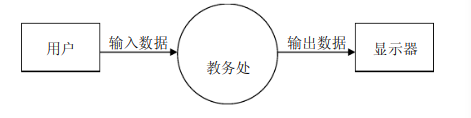
\includegraphics[width=0.7\textwidth]{选区_001} %插入图片,[]中设置图片大小,{}中是图片文件名
    \caption{总体流程} %最终文档中希望显示的图片标题
    \label{Fig.main2} %用于文内引用的标签
\end{figure}

\subsection{客户端基本流程}
\begin{figure}[H] %H为当前位置,!htb为忽略美学标准,htbp为浮动图形
    \centering %图片居中
    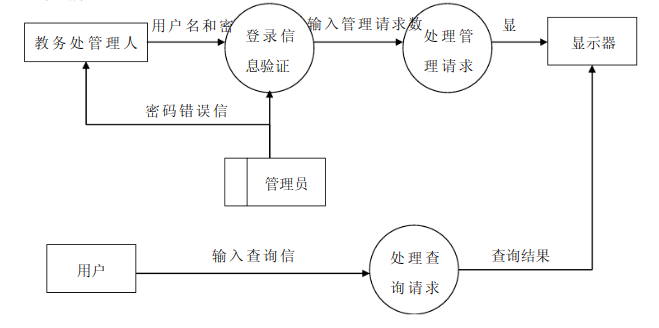
\includegraphics[width=0.7\textwidth]{选区_002} %插入图片,[]中设置图片大小,{}中是图片文件名
    \caption{客户端基本流程} %最终文档中希望显示的图片标题
    \label{Fig.main2} %用于文内引用的标签
\end{figure}

\subsection{服务器端基本流程}
\begin{figure}[H] %H为当前位置,!htb为忽略美学标准,htbp为浮动图形
    \centering %图片居中
    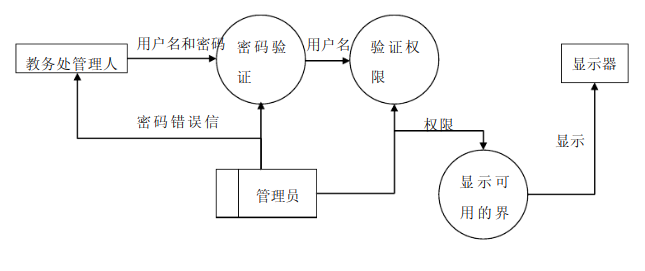
\includegraphics[width=0.7\textwidth]{选区_003} %插入图片,[]中设置图片大小,{}中是图片文件名
    \caption{服务端基本流程} %最终文档中希望显示的图片标题
    \label{Fig.main2} %用于文内引用的标签
\end{figure}

\subsection{基础数据管理}
“基础数据管理”功能模块用于维护整个教务系统正常运行所需的基础数据集,以保证
教务系统有一个统一的标准的基础数据集,便于数据的共享使用,内容包括入学年份、学年学期、院系数据、专业设置等。

\subsection{“学生成绩管理”功能模块}
“学生成绩管理”功能模块用于学生成绩管理系统提供了强大的学生成绩管理管理功能,对学生的各个学期的学生成绩进行保存记录。对学生成绩等信息的添加.修改.删除.查询.汇总.统计等操作。

\subsection{“学籍管理”功能模块}
“学籍管理”主要包括了高校学籍管理的常用信息,提供对学生学籍基本信息录入、查询、修改、打印输出、维护等常用功能,并提供学号编排、学生照片输入与显示、学籍变动(留级、休学、跳级、转班、转学、退学等)、奖惩登记、毕业情况

\subsection{“教室安排”功能模块}
“排课选课管理”功能模块用于根据教学计划、教室资源、教师资源等,制定每学期的课程表。用于对某学期全校课程进行设置,如课表统一制定、每天上课节数、统一的排课时段进行设置。对某个班级某学期具体开设的课程分别进行排课时段、单双周、连常课等特殊情况设置

\subsection{“考务成绩管理”功能模块}
“考务成绩管理”功能模块用于根据课程自动生成本学期的考试地点、考试时间、监考老师等数据,并对考试的过程和结果进行监控。“考务住处发布”用于发布考务信息,如学年、学期、期中(期末)考试、考试时间等,以及其他一些有关考务的事项。 “考试日程安排“用于对评卷专业、评卷科目、评卷教师、评卷日期、时间等评卷信息进行管理。“学生成绩录入”用于授课教师输入学生的考试成绩。(学生学籍信息表)

\subsection{“学生选课”功能模块}
“学生选课”功能模块用于对在校学生个学期的选课情况记录,包括所选课程、教室 安排、选课时间(学期)、选修的课程所在教室、以及对各个选修的课程的成绩记录修改等内容

\section{总体功能结构设计}
\begin{figure}[H] %H为当前位置,!htb为忽略美学标准,htbp为浮动图形
    \centering %图片居中
    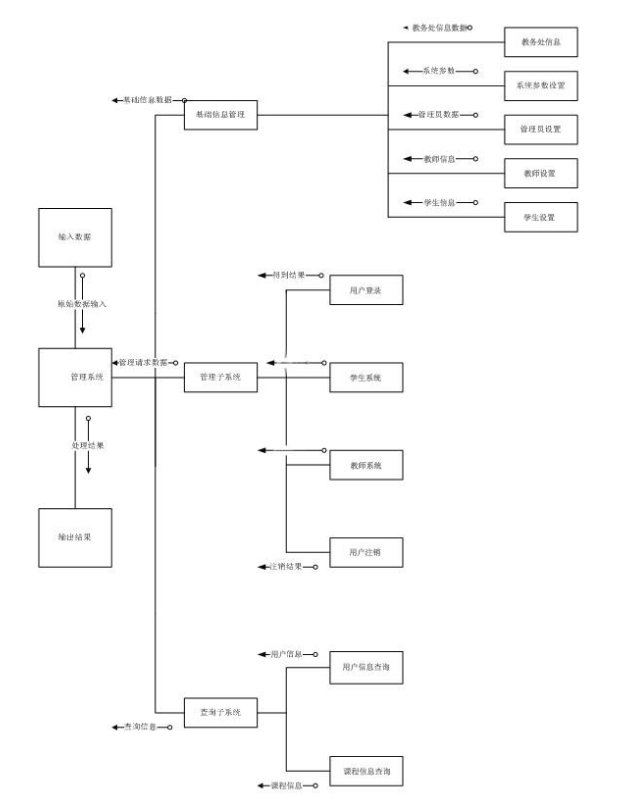
\includegraphics[width=0.7\textwidth]{选区_005} %插入图片,[]中设置图片大小,{}中是图片文件名
    \caption{总体功能结构设计} %最终文档中希望显示的图片标题
    \label{Fig.main2} %用于文内引用的标签
\end{figure}


\chapter{接口设计}
\section{外部接口}
比如说需要用到支付宝等外部支付系统,接口应当如何封装。

\subsection{支付宝接口}
详细讲述不同的接口(查询状态、支付交易、获取回执等)

\section{内部接口}
内部模块/系统之间的交互的接口。
\chapter{数据结构设计}
\section{用户管理系统数据结构设计}
需要学生个人信息表、教师信息表、科目信息表、开课结果信息表、成绩表

\section{物理结构设计}
无

\section{数据结构}
\begin{figure}[H] %H为当前位置,!htb为忽略美学标准,htbp为浮动图形
    \centering %图片居中
    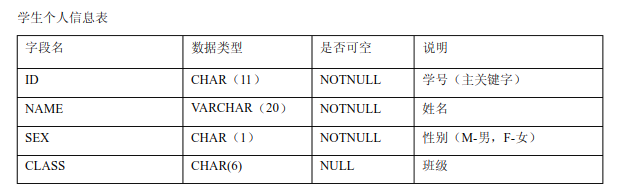
\includegraphics[width=0.7\textwidth]{选区_006} %插入图片,[]中设置图片大小,{}中是图片文件名
    \caption{学生个人信息表} %最终文档中希望显示的图片标题
    \label{Fig.main2} %用于文内引用的标签
\end{figure}

\begin{figure}[H] %H为当前位置,!htb为忽略美学标准,htbp为浮动图形
    \centering %图片居中
    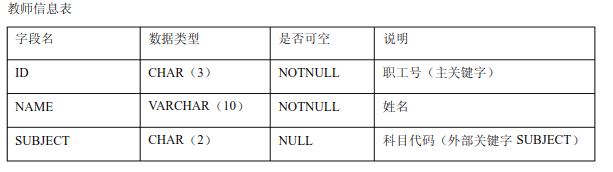
\includegraphics[width=0.7\textwidth]{选区_007} %插入图片,[]中设置图片大小,{}中是图片文件名
    \caption{教师信息表} %最终文档中希望显示的图片标题
    \label{Fig.main2} %用于文内引用的标签
\end{figure}

\begin{figure}[H] %H为当前位置,!htb为忽略美学标准,htbp为浮动图形
    \centering %图片居中
    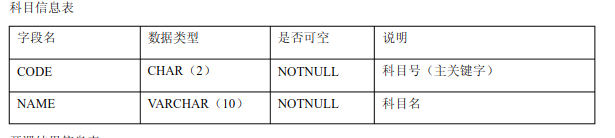
\includegraphics[width=0.7\textwidth]{选区_008} %插入图片,[]中设置图片大小,{}中是图片文件名
    \caption{科目信息表} %最终文档中希望显示的图片标题
    \label{Fig.main2} %用于文内引用的标签
\end{figure}

\begin{figure}[H] %H为当前位置,!htb为忽略美学标准,htbp为浮动图形
    \centering %图片居中
    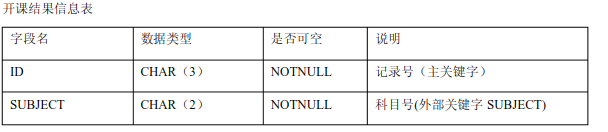
\includegraphics[width=0.7\textwidth]{选区_009} %插入图片,[]中设置图片大小,{}中是图片文件名
    \caption{开课结果信息表} %最终文档中希望显示的图片标题
    \label{Fig.main2} %用于文内引用的标签
\end{figure}

\begin{figure}[H] %H为当前位置,!htb为忽略美学标准,htbp为浮动图形
    \centering %图片居中
    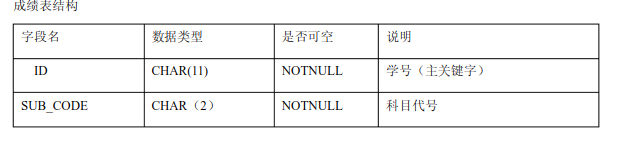
\includegraphics[width=0.7\textwidth]{选区_010} %插入图片,[]中设置图片大小,{}中是图片文件名
    \caption{成绩表} %最终文档中希望显示的图片标题
    \label{Fig.main2} %用于文内引用的标签
\end{figure}

\chapter{数据库设计}
\section{数据库环境说明}
本系统的数据系统采用MySQL/PostgreSQL/Microsoft SQL Server数据库系统。

其中xxx模块因为xxx而需要用到Hadoop架构。

\section{数据库的命名规则}
是否允许单词缩写,允许的单词缩写有哪些。

表名是单数还是复数。关联表如何命名。字符数限制等。

字段是否带上前缀(如integer类型则加上i前缀等)。

\section{逻辑设计}
是否需要满足某一种范式。

画个实体的逻辑关系表/图在此处。

\section{物理设计}
\subsection{数据库产品}
用哪家数据库,是否分布式等。
\subsection{实体属性、类型、精度}
\subsubsection{客户数据表设计}
\begin{table}[htbp]
\centering
\caption{用户数据表Users设计} \label{tab:client-database}
\begin{tabular}{|c|c|c|c|c|}
    \hline
    字段名 & 类型 & 大小 & 说明 & 备注 \\
    \hline
    ID & char & 64 & 用户的唯一标识符 & 主键\\
    \hline
    pw & char & 512 & 用户的登录密码 & · \\
    \hline
\end{tabular}
\note{用户数据表Users设计}
\end{table}

\subsubsection{订单数据表设计}
\begin{table}[htbp]
\centering
\caption{订单数据表Orders设计} \label{tab:order-database}
\begin{tabular}{|c|c|c|c|c|}
    \hline
    字段名 & 类型 & 大小 & 说明 & 备注 \\
    \hline
    ID & char & 64 & 订单的唯一标识符 & 主键\\
    \hline
    user & char & 64 & 对应用户 & 外键,来自xx表 \\
    \hline
\end{tabular}
\note{订单数据表Orders设计}
\end{table}
\section{安全性设计}
备份和容灾设计。

\section{数据库管理与维护说明}
对于数据库的维护,随时对数据库中的信息加以调试和保存备份。同样需要个工作人员进行系统的分析和用户的反馈,对系统进行升级以及功能的完善。同时保证系统安全有序的运行。
\chapter{界面设计}
\section{客户端界面}
此处应当有一个简略的图,重点是展示你与用户交互的逻辑。(processon上画一个不花时间)

\section{服务器端界面}
此处应当有一个简略的图。

\section{登录界面}
此处应当有一个简略的图。

\section{xxx功能界面}
此处应当有一个简略的图。

\chapter{出错处理设计}
\section{数据库出错处理}
多重备份时,应采取何种策略,先利用哪一份备份;系统是否暂停服务等。

\section{某模块失效处理}
是否整个系统暂停服务,还是维持最小服务状态、如何尽快恢复服务还是删库跑路等。
\chapter{安全保密设计}
数据保密: 由于我们这个软件是面向教务处管理的,里面会有很多重要数据。这些数据 不宜被外人知道,所以我们设计了登陆系统,保证了合法性。

操作安全: 由于操作不慎可能导致数据被误删,误改等情况,这里我们在每次删除的时 候提醒用户,以防误操作。

可能的内容包括保密性、是否采取加密传输、密钥如何分发和管理等。
\chapter{维护设计}
软件的维护主要包括,数据库的维护和软件功能的维护。 对于数据库的维护,本软件已经提供了数据库的备份和恢复的功能,可以方便的实现数据库的维护管理。 对于软件功能方面的维护,由于我们采用的是模块化的设计方法,每个模块(窗口)之间相互独立性较高,这样对软件的维护带来了很大的方便,对于单独功能的修改只需修改一个窗口就行了。


\chapter{图片}
本章展示图片相关用法。

\section{示例}
\begin{figure}[ht]
\centering

\includegraphics[width=10cm]{ustc_logo_fig}
\caption{测试图片} \label{fig:figure1}
\end{figure}

\section{带图注的图}
\begin{figure}[ht]
\centering

\includegraphics[width=10cm]{ustc_logo_fig}
\caption{带图注的图片}\label{fig:noted-figure}
\note{the solid lines represent the time histogram of the spontaneous activities of an old monkey cell(gray) and a young monkey cell (black). The bin-width is 1}
\end{figure}

\chapter{表格}

\section{A Simple Table}
\begin{table}[htbp]
\centering
\caption{这里是表的标题} \label{tab:simpletable}
\begin{tabular}{|c|c|}
    \hline
    a & b \\
    \hline
    c & d \\
    \hline
\end{tabular}
\note{这里是表的注释}
\end{table}

\section{长表格}
\begin{longtable}{ccc}
% 首页表头
\caption[长表格演示]{长表格演示} \label{tab:longtable} \\
\toprule[1.5pt]
名称  & 说明 & 备注\\
\midrule[1pt]
\endfirsthead
% 续页表头
\caption[]{长表格演示(续)} \\
\toprule[1.5pt]
名称  & 说明 & 备注 \\
\midrule[1pt]
\endhead
% 首页表尾
\hline
\multicolumn{3}{r}{\small 续下页}
\endfoot
% 续页表尾
\bottomrule[1.5pt]
\endlastfoot

AAAAAAAAAAAA   &   BBBBBBBBBBB   &   CCCCCCCCCCCCCC   \\
AAAAAAAAAAAA   &   BBBBBBBBBBB   &   CCCCCCCCCCCCCC   \\
AAAAAAAAAAAA   &   BBBBBBBBBBB   &   CCCCCCCCCCCCCC   \\
AAAAAAAAAAAA   &   BBBBBBBBBBB   &   CCCCCCCCCCCCCC   \\
AAAAAAAAAAAA   &   BBBBBBBBBBB   &   CCCCCCCCCCCCCC   \\
AAAAAAAAAAAA   &   BBBBBBBBBBB   &   CCCCCCCCCCCCCC   \\
AAAAAAAAAAAA   &   BBBBBBBBBBB   &   CCCCCCCCCCCCCC   \\
AAAAAAAAAAAA   &   BBBBBBBBBBB   &   CCCCCCCCCCCCCC   \\
AAAAAAAAAAAA   &   BBBBBBBBBBB   &   CCCCCCCCCCCCCC   \\
AAAAAAAAAAAA   &   BBBBBBBBBBB   &   CCCCCCCCCCCCCC   \\
AAAAAAAAAAAA   &   BBBBBBBBBBB   &   CCCCCCCCCCCCCC   \\
AAAAAAAAAAAA   &   BBBBBBBBBBB   &   CCCCCCCCCCCCCC   \\
AAAAAAAAAAAA   &   BBBBBBBBBBB   &   CCCCCCCCCCCCCC   \\
AAAAAAAAAAAA   &   BBBBBBBBBBB   &   CCCCCCCCCCCCCC   \\
AAAAAAAAAAAA   &   BBBBBBBBBBB   &   CCCCCCCCCCCCCC   \\
AAAAAAAAAAAA   &   BBBBBBBBBBB   &   CCCCCCCCCCCCCC   \\
AAAAAAAAAAAA   &   BBBBBBBBBBB   &   CCCCCCCCCCCCCC   \\
AAAAAAAAAAAA   &   BBBBBBBBBBB   &   CCCCCCCCCCCCCC   \\
AAAAAAAAAAAA   &   BBBBBBBBBBB   &   CCCCCCCCCCCCCC   \\
AAAAAAAAAAAA   &   BBBBBBBBBBB   &   CCCCCCCCCCCCCC   \\
AAAAAAAAAAAA   &   BBBBBBBBBBB   &   CCCCCCCCCCCCCC   \\
AAAAAAAAAAAA   &   BBBBBBBBBBB   &   CCCCCCCCCCCCCC   \\
AAAAAAAAAAAA   &   BBBBBBBBBBB   &   CCCCCCCCCCCCCC   \\
AAAAAAAAAAAA   &   BBBBBBBBBBB   &   CCCCCCCCCCCCCC   \\
AAAAAAAAAAAA   &   BBBBBBBBBBB   &   CCCCCCCCCCCCCC   \\
AAAAAAAAAAAA   &   BBBBBBBBBBB   &   CCCCCCCCCCCCCC   \\
AAAAAAAAAAAA   &   BBBBBBBBBBB   &   CCCCCCCCCCCCCC   \\
AAAAAAAAAAAA   &   BBBBBBBBBBB   &   CCCCCCCCCCCCCC   \\
AAAAAAAAAAAA   &   BBBBBBBBBBB   &   CCCCCCCCCCCCCC   \\
AAAAAAAAAAAA   &   BBBBBBBBBBB   &   CCCCCCCCCCCCCC   \\
AAAAAAAAAAAA   &   BBBBBBBBBBB   &   CCCCCCCCCCCCCC   \\
AAAAAAAAAAAA   &   BBBBBBBBBBB   &   CCCCCCCCCCCCCC   \\
AAAAAAAAAAAA   &   BBBBBBBBBBB   &   CCCCCCCCCCCCCC   \\
AAAAAAAAAAAA   &   BBBBBBBBBBB   &   CCCCCCCCCCCCCC   \\
AAAAAAAAAAAA   &   BBBBBBBBBBB   &   CCCCCCCCCCCCCC   \\
AAAAAAAAAAAA   &   BBBBBBBBBBB   &   CCCCCCCCCCCCCC   \\
\end{longtable}

\chapter{算法环境}
模板中使用 \texttt{algorithm2e} 宏包实现算法环境。关于该宏包的具体用法,
请阅读宏包的官方文档。

\begin{algorithm}[htbp]
\SetAlgoLined
\KwData{this text}
\KwResult{how to write algorithm with \LaTeX2e }

initialization\;
\While{not at end of this document}{
    read current\;
    \eIf{understand}{
        go to next section\;
        current section becomes this one\;
    }{
        go back to the beginning of current section\;
    }
}
\caption{算法示例1}
\label{algo:algorithm1}
\end{algorithm}

\IncMargin{1em}
\begin{algorithm}
\SetKwData{Left}{left}\SetKwData{This}{this}\SetKwData{Up}{up}
\SetKwFunction{Union}{Union}\SetKwFunction{FindCompress}{FindCompress}
\SetKwInOut{Input}{input}\SetKwInOut{Output}{output}

\Input{A bitmap $Im$ of size $w\times l$}
\Output{A partition of the bitmap}
\BlankLine
\emph{special treatment of the first line}\;
\For{$i\leftarrow 2$ \KwTo $l$}{
    \emph{special treatment of the first element of line $i$}\;
    \For{$j\leftarrow 2$ \KwTo $w$}{\label{forins}
        \Left$\leftarrow$ \FindCompress{$Im[i,j-1]$}\;
        \Up$\leftarrow$ \FindCompress{$Im[i-1,]$}\;
        \This$\leftarrow$ \FindCompress{$Im[i,j]$}\;
        \If(\tcp*[h]{O(\Left,\This)==1}){\Left compatible with \This}{\label{lt}
            \lIf{\Left $<$ \This}{\Union{\Left,\This}}
            \lElse{\Union{\This,\Left}}
        }
        \If(\tcp*[f]{O(\Up,\This)==1}){\Up compatible with \This}{\label{ut}
        \lIf{\Up $<$ \This}{\Union{\Up,\This}}
        \tcp{\This is put under \Up to keep tree as flat as possible}\label{cmt}
        \lElse{\Union{\This,\Up}}\tcp*[h]{\This linked to \Up}\label{lelse}
        }
    }
    \lForEach{element $e$ of the line $i$}{\FindCompress{p}}
}
\caption{算法示例2}\label{algo_disjdecomp}
\label{alog:algorithm2}
\end{algorithm}\DecMargin{1em}

\chapter{代码环境}
模板中使用 \texttt{listings} 宏包实现代码环境。详细用法见宏包的官方说明文档。

以下是代码示例,可以在文中任意位置引用\autoref{first-code} 。
\begin{lstlisting}[language=C, caption=示例代码, label={code:first-code}]
#include <stdio.h>

int main( )
{
    printf("hello, world\n");
    return 0;
}
\end{lstlisting}

\chapter{引用文献标注}

\section{著者-出版年制标注法}

\noindent
\verb|\citestyle{ustcauthoryear}|
\citestyle{ustcauthoryear}

\noindent
\begin{tabular}{l@{\quad$\Rightarrow$\quad}l}
  \verb|\cite{knuth86a}| & \cite{knuth86a}\\
  \verb|\citet{knuth86a}| & \citet{knuth86a}\\
  \verb|\citet[chap.~2]{knuth86a}| & \citet[chap.~2]{knuth86a}\\[0.5ex]
  \verb|\citep{knuth86a}| & \citep{knuth86a}\\
  \verb|\citep[chap.~2]{knuth86a}| & \citep[chap.~2]{knuth86a}\\
  \verb|\citep[see][]{knuth86a}| & \citep[see][]{knuth86a}\\
  \verb|\citep[see][chap.~2]{knuth86a}| & \citep[see][chap.~2]{knuth86a}\\[0.5ex]
  \verb|\citet*{knuth86a}| & \citet*{knuth86a}\\
  \verb|\citep*{knuth86a}| & \citep*{knuth86a}\\
\end{tabular}

\noindent
\begin{tabular}{l@{\quad$\Rightarrow$\quad}l}
  \verb|\citet{knuth86a,tlc2}| & \citet{knuth86a,tlc2}\\
  \verb|\citep{knuth86a,tlc2}| & \citep{knuth86a,tlc2}\\
  \verb|\cite{knuth86a,knuth84}| & \cite{knuth86a,knuth84}\\
  \verb|\citet{knuth86a,knuth84}| & \citet{knuth86a,knuth84}\\
  \verb|\citep{knuth86a,knuth84}| & \citep{knuth86a,knuth84}\\
\end{tabular}

\section{顺序编码制标注法}

\noindent
\verb|\citestyle{ustcnumerical}|
\citestyle{ustcnumerical}

\noindent
\begin{tabular}{l@{\quad$\Rightarrow$\quad}l}
  \verb|\cite{knuth86a}| & \cite{knuth86a}\\
  \verb|\citet{knuth86a}| & \citet{knuth86a}\\
  \verb|\citet[chap.~2]{knuth86a}| & \citet[chap.~2]{knuth86a}\\[0.5ex]
  \verb|\citep{knuth86a}| & \citep{knuth86a}\\
  \verb|\citep[chap.~2]{knuth86a}| & \citep[chap.~2]{knuth86a}\\
  \verb|\citep[see][]{knuth86a}| & \citep[see][]{knuth86a}\\
  \verb|\citep[see][chap.~2]{knuth86a}| & \citep[see][chap.~2]{knuth86a}\\[0.5ex]
  \verb|\citet*{knuth86a}| & \citet*{knuth86a}\\
  \verb|\citep*{knuth86a}| & \citep*{knuth86a}\\
\end{tabular}

\noindent
\begin{tabular}{l@{\quad$\Rightarrow$\quad}l}
  \verb|\citet{knuth86a,tlc2}| & \citet{knuth86a,tlc2}\\
  \verb|\citep{knuth86a,tlc2}| & \citep{knuth86a,tlc2}\\
  \verb|\cite{knuth86a,knuth84}| & \cite{knuth86a,knuth84}\\
  \verb|\citet{knuth86a,knuth84}| & \citet{knuth86a,knuth84}\\
  \verb|\citep{knuth86a,knuth84}| & \citep{knuth86a,knuth84}\\
  \verb|\cite{knuth86a,knuth84,tlc2}| & \cite{knuth86a,knuth84,tlc2}\\
\end{tabular}

\section{其他形式的标注}

\noindent
\begin{tabular}{l@{\quad$\Rightarrow$\quad}l}
  \verb|\citealt{tlc2}| & \citealt{tlc2}\\
  \verb|\citealt*{tlc2}| & \citealt*{tlc2}\\
  \verb|\citealp{tlc2}| & \citealp{tlc2}\\
  \verb|\citealp*{tlc2}| & \citealp*{tlc2}\\
  \verb|\citealp{tlc2,knuth86a}| & \citealp{tlc2,knuth86a}\\
  \verb|\citealp[pg.~32]{tlc2}| & \citealp[pg.~32]{tlc2}\\
  \verb|\citenum{tlc2}| & \citenum{tlc2}\\
  \verb|\citetext{priv.\ comm.}| & \citetext{priv.\ comm.}\\
\end{tabular}

\noindent
\begin{tabular}{l@{\quad$\Rightarrow$\quad}l}
  \verb|\citeauthor{tlc2}| & \citeauthor{tlc2}\\
  \verb|\citeauthor*{tlc2}| & \citeauthor*{tlc2}\\
  \verb|\citeyear{tlc2}| & \citeyear{tlc2}\\
  \verb|\citeyearpar{tlc2}| & \citeyearpar{tlc2}\\
\end{tabular}

\bibliography{bib/tex}


\end{document}
